%%%%%%%%%%%%%%%%%%%%%%%%%%%%%%%%%%%%%%%%%%%%%%%
%%%     Declarations (skip to Begin Document, line 88, for parts you fill in)
%%%%%%%%%%%%%%%%%%%%%%%%%%%%%%%%%%%%%%%%%%%%%%%

\documentclass[10pt]{article}

\usepackage{geometry}  % Lots of layout options.  See http://en.wikibooks.org/wiki/LaTeX/Page_Layout
\geometry{letterpaper}  % ... or a4paper or a5paper or ... 
\usepackage{fullpage}  % somewhat standardized smaller margins (around an inch)
\usepackage{setspace}  % control line spacing in latex documents
\usepackage[parfill]{parskip}  % Activate to begin paragraphs with an empty line rather than an indent

\usepackage{amsmath,amssymb}  % latex math
\usepackage{empheq} % http://www.ctan.org/pkg/empheq
\usepackage{bm,upgreek}  % allows you to write bold greek letters (upper & lower case)

% for typsetting algorithm pseudocode see http://en.wikibooks.org/wiki/LaTeX/Algorithms_and_Pseudocode
\usepackage{algorithmic,algorithm}  

\usepackage{graphicx}  % inclusion of graphics; see: http://en.wikibooks.org/wiki/LaTeX/Importing_Graphics
% allow easy inclusion of .tif, .png graphics
\DeclareGraphicsRule{.tif}{png}{.png}{`convert #1 `dirname #1`/`basename #1 .tif`.png}

% \usepackage{subfigure}  % allows subfigures in figure
\usepackage{caption}
\usepackage{subcaption}

\usepackage{xspace}
\newcommand{\latex}{\LaTeX\xspace}

\usepackage{color}  % http://en.wikibooks.org/wiki/LaTeX/Colors

\long\def\todo#1{{\color{red}{\bf TODO: #1}}}

\long\def\ans#1{{\color{blue}{\em #1}}}
\long\def\ansnem#1{{\color{blue}#1}}
\long\def\boldred#1{{\color{red}{\bf #1}}}
\long\def\boldred#1{\textcolor{red}{\bf #1}}
\long\def\boldblue#1{\textcolor{blue}{\bf #1}}

% Useful package for syntax highlighting of specific code (such as python) -- see below
\usepackage{listings}  % http://en.wikibooks.org/wiki/LaTeX/Packages/Listings
\usepackage{textcomp}

%%% The following lines set up using the listings package
\renewcommand{\lstlistlistingname}{Code Listings}
\renewcommand{\lstlistingname}{Code Listing}

%%% Specific for python listings
\definecolor{gray}{gray}{0.5}
\definecolor{green}{rgb}{0,0.5,0}

\lstnewenvironment{python}[1][]{
\lstset{
language=python,
basicstyle=\footnotesize,  % could also use this -- a little larger \ttfamily\small\setstretch{1},
stringstyle=\color{red},
showstringspaces=false,
alsoletter={1234567890},
otherkeywords={\ , \}, \{},
keywordstyle=\color{blue},
emph={access,and,break,class,continue,def,del,elif ,else,%
except,exec,finally,for,from,global,if,import,in,i s,%
lambda,not,or,pass,print,raise,return,try,while},
emphstyle=\color{black}\bfseries,
emph={[2]True, False, None, self},
emphstyle=[2]\color{green},
emph={[3]from, import, as},
emphstyle=[3]\color{blue},
upquote=true,
morecomment=[s]{"""}{"""},
commentstyle=\color{gray}\slshape,
emph={[4]1, 2, 3, 4, 5, 6, 7, 8, 9, 0},
emphstyle=[4]\color{blue},
literate=*{:}{{\textcolor{blue}:}}{1}%
{=}{{\textcolor{blue}=}}{1}%
{-}{{\textcolor{blue}-}}{1}%
{+}{{\textcolor{blue}+}}{1}%
{*}{{\textcolor{blue}*}}{1}%
{!}{{\textcolor{blue}!}}{1}%
{(}{{\textcolor{blue}(}}{1}%
{)}{{\textcolor{blue})}}{1}%
{[}{{\textcolor{blue}[}}{1}%
{]}{{\textcolor{blue}]}}{1}%
{<}{{\textcolor{blue}<}}{1}%
{>}{{\textcolor{blue}>}}{1},%
%framexleftmargin=1mm, framextopmargin=1mm, frame=shadowbox, rulesepcolor=\color{blue},#1
framexleftmargin=1mm, framextopmargin=1mm, frame=single,#1
}}{}
%%% End python code listing definitions

\DeclareMathOperator{\diag}{diag}
\DeclareMathOperator{\cov}{cov}

%%%%%%%%%%%%%%%%%%%%%%%%%%%%%%%%%%%%%%%%%%%%%%%
%%%     Begin Document
%%%%%%%%%%%%%%%%%%%%%%%%%%%%%%%%%%%%%%%%%%%%%%%

\begin{document}

\begin{center}
    {\Large {\bf ISTA 421/521 -- Homework 5}} \\
    \boldred{Due: Wednesday, November 17, 5pm} \\
    25 pts total for Undergrads and Grads\\
    
\end{center}

\begin{flushright}
Perla Vanessa Jaime Gaytán %% Fill in your name here

Undergraduate  %% select which you are!
\end{flushright}

\vspace{1cm}
{\Large {\bf Instructions}}

In this assignment, exercises 2 and 3 require you to write small python scripts; the details are provided in those exercises.  All of the exercises in this homework require written derivations, so you will also submit a .pdf of your written answers.  (You can use \latex or any other system (including handwritten; plots, of course, must be program-generated) as long as the final version is in PDF.)

NOTE: In this assignment there are no separate "Graduate" exercises.

As in previous homework, pytest ``unit tests'' are provided to help guide your progress.

You may work with others in the course on the homework. However, if you do, you. {\bf must} list he names of everyone you worked with, along with which problems you collaborated. Your final submissions of code and written answers {\bf MUST ALL BE IN YOUR OWN CODE FORMULATION AND WORDS}; you cannot submit copies of the same work -- doing so will be considered cheating.

(FCMA refers to the course text: Rogers and Girolami (2016), {\em A First Course in Machine Learning}, second edition.  For general notes on using \latex to typeset math, see: \\{\tt http://en.wikibooks.org/wiki/LaTeX/Mathematics})
\vspace{.5cm}



%%%%%%%%%%%%%%%%
%%%     Exercises
%%%%%%%%%%%%%%%%

\newpage
\begin{itemize}


%%%     Exercise 1
\item[1.]  [8 points]
Adapted from {\bf Exercise 4.2} of FCMA p.163:

In Chapter 3, we computed the posterior density over $r$, the probability of a coin giving heads, using a beta prior and a binomial likelihood.  Recalling that the beta prior, with parameters $\alpha$ and $\beta$, is given by
\begin{eqnarray*}
p(r | \alpha, \beta) = \frac{\Gamma(\alpha + \beta)}{\Gamma(\alpha) \Gamma(\beta)} r^{\alpha - 1} (1 - r)^{\beta - 1}
\end{eqnarray*}
and the binomial likelihood, assuming $y$ heads in $N$ throws, is given by
\begin{eqnarray*}
p(y | r, N) = {N \choose y} r^{y} (1 - r)^{N-y} ~,
\end{eqnarray*}
{\bf compute the Laplace approximation to the posterior}.  (Note, you should be able to obtain a closed-form solution for the MAP value, $\hat{r}$, by getting the log posterior, differentiating (with respect to $r$), equating to zero and solving for $r$.)

{\bf Solution.}
\begin{figure}[H]
\begin{center}
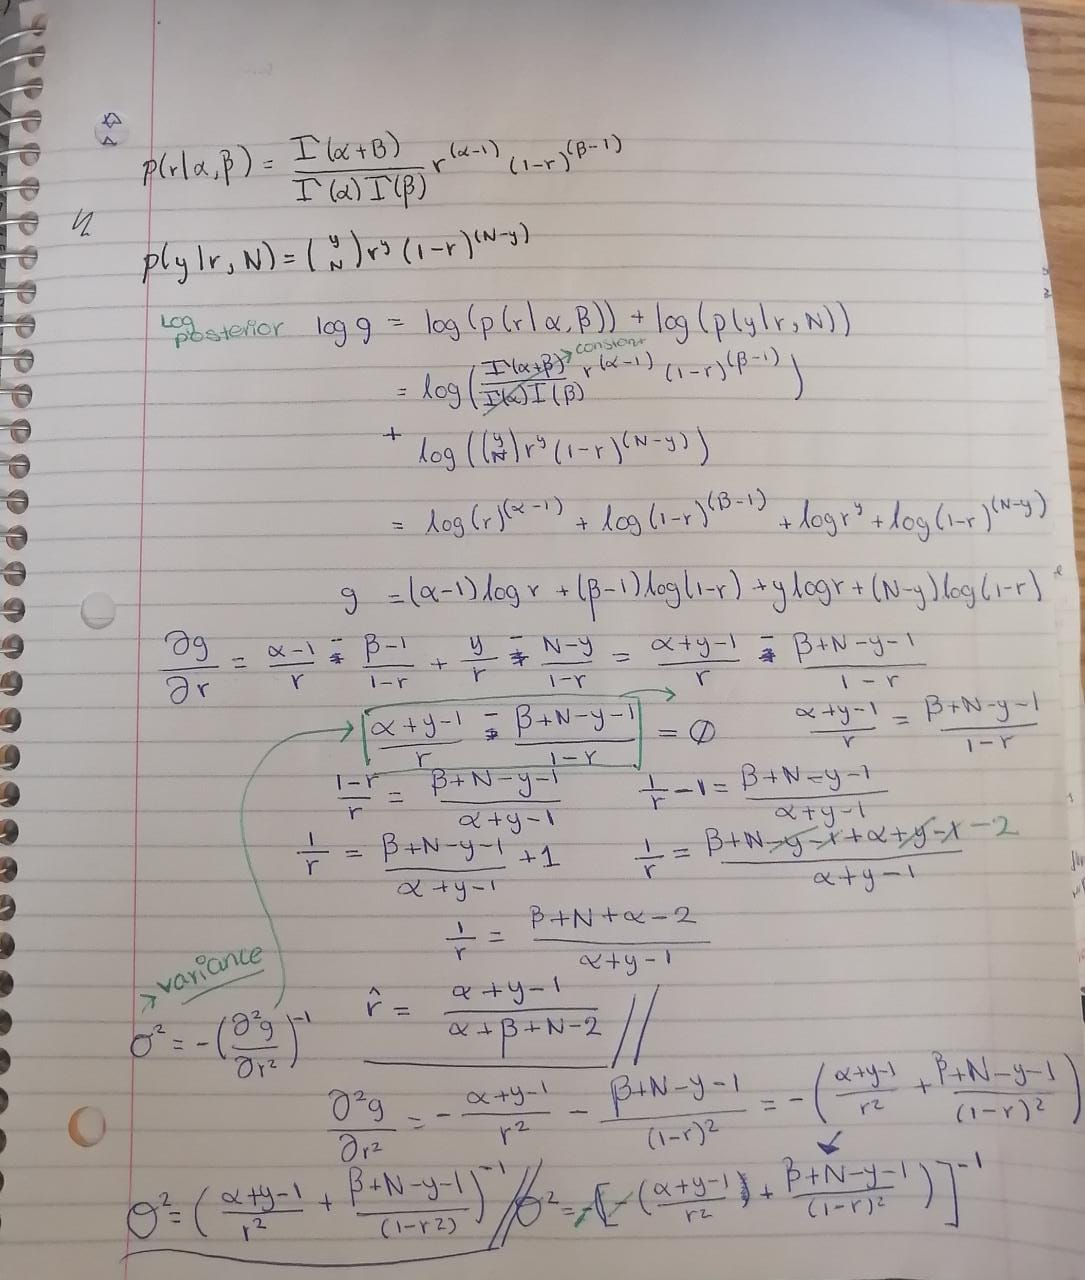
\includegraphics[width=.7\textwidth]{figures/ex1.jpeg}
\caption{Written solution to Exercise 1.}
\end{center}
\end{figure}


%%%     Exercise 2
\item[2.]  [4 points]
Adapted from {\bf Exercise 4.3} of FCMA p.163:

In the previous exercise you computed the Laplace approximation to the true beta posterior.  In this exercise, you will implement the calculation of the posterior Beta parameters and the computation of the Laplace approximation parameters in the function {\tt plot\_laplace\_approx} in the provided file {\tt laplace\_approx.py}. Once implemented, running the script (set {\tt RUN\_LAPLACE\_APPROX} to {\tt True}) will plot both the true Beta posterior and the Laplace approximation for the following three parameter settings:
\begin{enumerate}
\item $\alpha = 5$, $\beta = 5$, $N = 20$, and $y = 10$,
\item $\alpha = 3$, $\beta = 15$, $N = 10$, and $y = 3$,
\item $\alpha = 1$, $\beta = 30$, $N = 10$, and $y = 3$.
\end{enumerate}
This will produce three separate plots (each with the Beta and associated Laplace approximation). Include these in your written answer and be sure to clearly indicate in your plot captions the parameter values that were used to generate the curves in the plot. In your written answer, also include how the two distributions (the true Beta posterior and the Laplace approximation) compare in each case. NOTE: {\tt scipy.stats.normal} expects the scale parameter to be the standard deviation (i.e., take the square root, {\tt math.sqrt(x)}, of the variance you compute for the Laplace approximation.

{\bf Solution.}
%%% For Latex Users:
\begin{figure}[h!]
\centering
\begin{subfigure}[]{.32\textwidth}
  \centering
  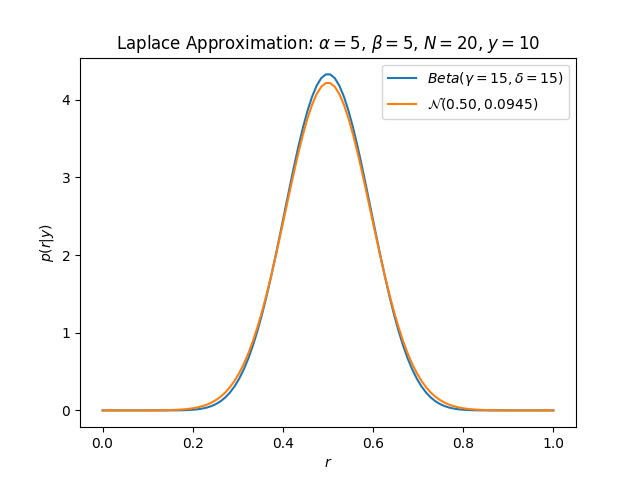
\includegraphics[width=1\linewidth]{figures/laplace_case1.png}
  \caption{$\alpha = 5$, $\beta = 5$, $N = 20$, and $y = 10$}
  \label{fig:sub1}
\end{subfigure}
\begin{subfigure}{.32\textwidth}
  \centering
  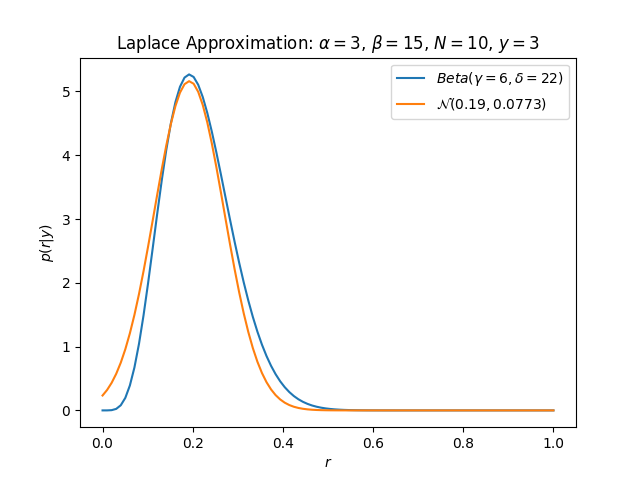
\includegraphics[width=1\linewidth]{figures/laplace_case2.png}
  \caption{$\alpha = 3$, $\beta = 15$, $N = 10$, and $y = 3$}
  \label{fig:sub2}
\end{subfigure}
\begin{subfigure}{.32\textwidth}
  \centering
  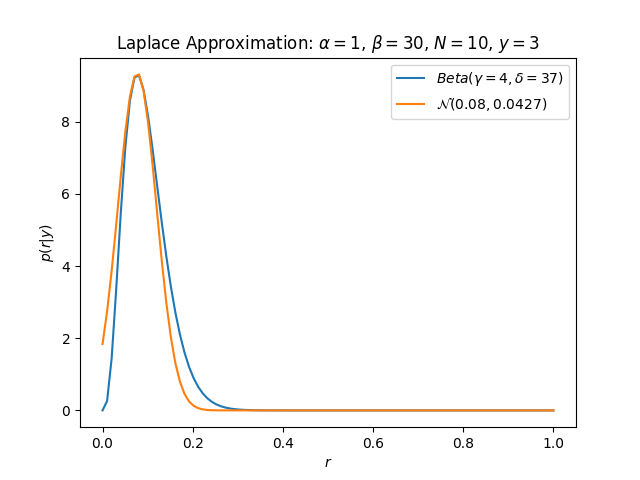
\includegraphics[width=1\linewidth]{figures/laplace_case3.png}
  \caption{$\alpha = 1$, $\beta = 30$, $N = 10$, and $y = 3$}
  \label{fig:sub3}
\end{subfigure}
\caption{Beta and Associated Laplace Approximation.}
\label{fig:laplace}
\end{figure}
\\
The Laplace approximation approximates the posterior with a Gaussian which is better whenever we want to approximate to a value. The true posterior is better to compute expectations. They don't look too different from each other. 
%In your written answer, also include how the two distributions (the true %Beta posterior and the Laplace approximation) compare in each case.

%%%     Problem 3
\item[3.]  [5 points]
Adapted from {\bf Exercise 4.4} of FCMA p.164:

Given the expression for the area of a circle, $A = \pi r^2$, and {\em using only uniformly distributed random variates}, that is, using only uniform random number draws computed by python's {\tt random.uniform}, devise a sampling approach for estimating $\pi$.  (Just to state the obvious: you are not allowed to use any other direct numeric representation of $\pi$, such as {\tt math.pi}, in your solution.) In your written answer, describe your method in detail. Implement your method in the function {\tt estimate\_pi} in {\tt pi\_sample\_estimate.py}. This function takes a single argument, $N$, representing the number of samples to be used in your estimate. In your written answer, give your estimate based on 1 million samples to 6 decimal places. The provided unit test expects that your estimate will be within $0.005$ of $\pi$ (more specifically, the approximation of {\tt math.pi}) when based on $1,000,000$ (one million) samples. Since this is a sampling method, it is possible for a good solution to this exercise to still get an unlikely sample that is outside of $0.005$ of $\pi$, however this is expected to be rare; with a good solution, you should almost always pass the unit test. (NOTE: You do {\em not} need to use Metropolis-Hastings to compute this.)
\\
\\
\\
{\bf Solution.} %$<$Solution goes here$>$ 
\\
I sample pairs of random values from a uniform distribution. The probability that one of this points is inside of the circle is the same as the ratio of the area of the circle and the area of the square of with the length of the same ratio. We can get an estimate by generating ({\it N}) pairs and obtaining how many of these pairs lies inside the circle ({\it n}). We can get an approximation of $\pi$ by dividing {\it n} into the number of samples({\it N}) multiply by $0.5^2$.
\begin{eqnarray*}
\pi &=& \frac{n}{0.5^2N}
\end{eqnarray*}



%%%     Exercise 4
\item[4.]  [8 points]
Adapted from {\bf Exercise 4.6} of FCMA p.164:

Assume that we observe $N$ vectors of attributes, $\mathbf{x}_1, ..., \mathbf{x}_N$, and associated integer counts $t_1, ..., t_N$.  A Poisson likelihood would be suitable:
\begin{eqnarray*}
p(t_n | \mathbf{x}_n, \mathbf{w}) = \frac{f(\mathbf{x}_n; \mathbf{w})^{t_n} \exp \{ -f(\mathbf{x}_n; \mathbf{w}) \}}{t_n!},
\end{eqnarray*}
where $f(\mathbf{x}_n;\mathbf{w}) = \mathbf{w}^\top\mathbf{x}_n$.
Assuming a zero-mean Gaussian prior on $\mathbf{w}$ with constant diagonal covariance of $\sigma^2$, derive the gradient and Hessian of the posterior.  Using these, express the parameter update rules for (a) gradient {\em ascent} (because we're maximizing) update (in class we looked at Widrow-Hoff, which is typically expressed for {\em descent}), and (b) Newton-Raphson.

The following facts will help in the derivation.  
First, keep in mind that although $\mathbf{w}$ and $\mathbf{x}_n$ are vectors (of the same dimension), their dot product, $\mathbf{w}^\top\mathbf{x}_n$, is a {\em scalar} value.  This means you can take the partial derivative of $\log \mathbf{w}^\top\mathbf{x}_n$ with respect to $\mathbf{w}$.  
Second, here's a little more detail on taking the vector second derivative to get the Hessian. The Hessian is a matrix representing the second partial derivatives of the gradient with respect to itself (see Comment 2.6 of p.73), and the second derivative will involve the {\em transpose} of the partial derivative with respect to $\mathbf{w}$. That is, first you will take the partial with respect to $\mathbf{w}$ to get the gradient (used for the first part of the exercise, for deriving the gradient ascent update) then you'll take the derivative of the gradient with respect to $\mathbf{w}^\top$. Taking the derivative with respect to $\mathbf{w}^\top$ works pretty much like taking the derivative with respect to $\mathbf{w}$, except the result will itself be transposed. The following shows examples of taking the derivative of $\mathbf{w}^\top \mathbf{x}_n$ with respect to $\mathbf{w}$ and separately with respect to $\mathbf{w}^\top$:
\begin{eqnarray*}
\frac{\partial (\mathbf{w}^\top \mathbf{x}_n)}{\partial \mathbf{w}} = \mathbf{x}_n
~~~~\mathrm{and}~~~~
\frac{\partial (\mathbf{w}^\top \mathbf{x}_n)}{\partial \mathbf{w}^\top} = \mathbf{x}_n^\top
\end{eqnarray*}
In this exercise, when you're computing the Hessian, you'll be taking the {\em second} partial derivative with respect to $\mathbf{w}$ of the product of the prior and likelihood (let's call that $g(\mathbf{w})$), first taking the partial with respect to $\mathbf{w}$ and then $\mathbf{w}^\top$:
\begin{eqnarray*}
\frac{\partial^2 g(\mathbf{w})}{\partial \mathbf{w} \partial \mathbf{w}^\top}
\end{eqnarray*}

{\bf Solution.}
\begin{figure}[H]
\begin{center}
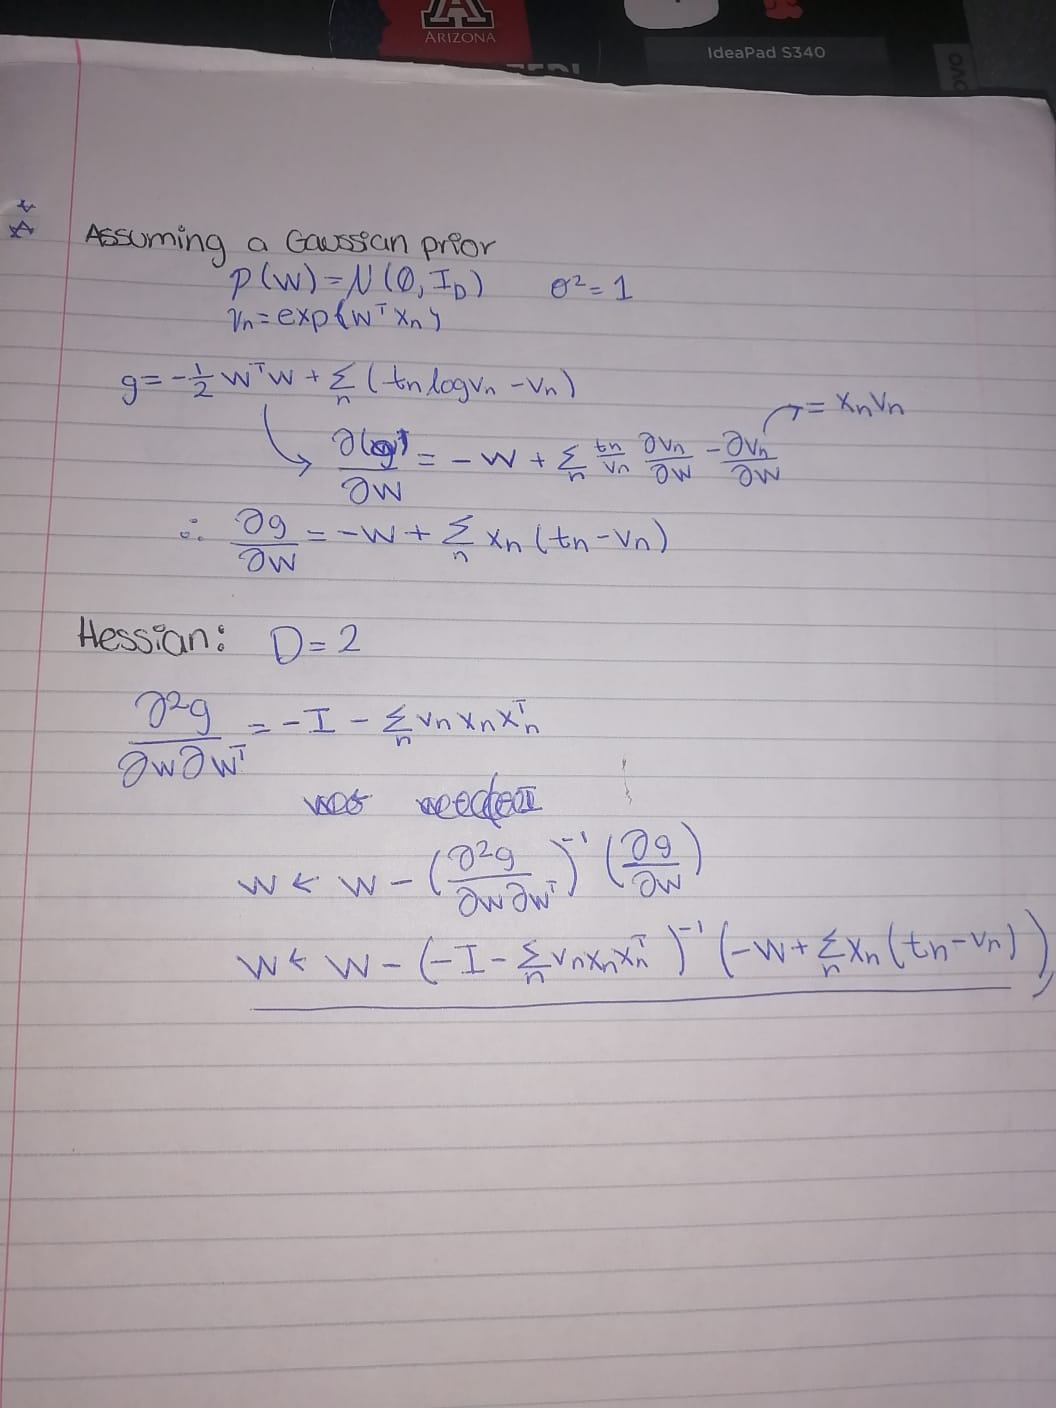
\includegraphics[width=.7\textwidth]{figures/ex4.jpeg}
\caption{Written solution to Exercise 4.}
\end{center}
\end{figure}

\end{itemize}

\end{document}

